
% This LaTeX was auto-generated from MATLAB code.
% To make changes, update the MATLAB code and republish this document.

\documentclass{article}
\usepackage{graphicx}
\usepackage{color}

\sloppy
\definecolor{lightgray}{gray}{0.5}
\setlength{\parindent}{0pt}

\begin{document}

    
    
\section*{}


\subsection*{Contents}

\begin{itemize}
\setlength{\itemsep}{-1ex}
   \item Macroeconomics assignment 1
   \item Question 1
   \item Comment: The time series plot for GDP, household consumption, government expenditure and investment shows the strong correlation between those time series. Consumption, investment, and government expenditure make up for about 52, 22 and 24 percent of GDP, respectively.
   \item Comment: The stationary (cyclical) component of GDP, consumption, investment, and government expenditure is obtained using the HP filter with a smoothing parameter of 1600. The cyclical components for each variable are then plotted on the same graph. The plot shows how each variable deviates from its long-term trend over time. The cyclical component is much smoother than the original time series and captures the long-term trends in the data. From the curves, it appears that investments is the most volatile time series among the four.
   \item Comment: The results indicate that the cyclical components of output (Y), consumption (C), investment (I), and government spending (G) have standard deviations ranging from 0.2112 to 0.2438, and relative standard deviations ranging from 1.7054\% to 2.1316\%. The contemporaneous output correlations of cyclical components suggest that there are high positive correlations among Y, C, I, and G, with correlation coefficients ranging from 0.9786 to 1.0000. This indicates that the cyclical fluctuations in these variables tend to move together. The relative standard deviation of investment is the highest among the four variables, at 2.1316\%. This suggests that investment is the most volatile of the four components. The relative standard deviation of consumption is slightly higher than that of output, at 1.7531\% and 1.7054\%, respectively. This suggests that consumption is also subject to some volatility, although less so than investment.
   \item Comment: The subsample analysis shows that cyclical components of output, consumption, investment, and government spending are highly correlated, with output and consumption being almost perfectly correlated. The relative standard deviation of the cyclical components for each variable is around 1.4\%. Compared to the results of the full sample, the subsample analysis shows a slightly lower degree of cyclical volatility.
   \item Comment: For subsample 2, the standard deviations of cyclical components are much lower than both the full sample and subsample 1. The relative standard deviations are also much lower for subsample 2. The contemporaneous output correlations of cyclical components for subsample 2 show higher correlation between Y and G compared to subsample 1, but lower correlation between Y and I. Overall, subsample 2 shows much lower volatility and correlation compared to the full sample and subsample 1.
\end{itemize}


\subsection*{Macroeconomics assignment 1}

\begin{verbatim}
title = 'Advanced Macroeconomics 2 Assignment 1';
author = 'Tim Koenders and Max Heinze';
fprintf('%s\n%s\n\n', title, author);
\end{verbatim}

        \color{lightgray} \begin{verbatim}Advanced Macroeconomics 2 Assignment 1
Tim Koenders and Max Heinze

\end{verbatim} \color{black}
    

\subsection*{Question 1}

\begin{verbatim}
% Read in macroeconomic data from an Excel file and prepare data
data=readtable("Data_Macro2_France.xlsx");
data.Year=datetime(data.TIME,'InputFormat','uuuu-QQQ','Format','uuuu-QQQ');
data_timetable = table2timetable(data, 'RowTimes', 'Year');
Y = data.GDP;
C = data.HouseholdConsumption;
I = data.CapitalFormation;
G = data.GovernmentConsumption;
Year = data.Year;
C = rmmissing(C);
I = rmmissing(I);
G = rmmissing(G);
% Remove the first 20 years of GDP data to make time series balanced (since they contain missing values)
Y(1:20) = [];
Year(1:20) = [];

%Calculating sample means and plotting the time series
C_Y = C ./ Y;
I_Y = I ./ Y;
G_Y = G ./ Y;
fprintf('Sample means:\n');
fprintf('C/Y: %.4f\n', mean(C_Y));
fprintf('I/Y: %.4f\n', mean(I_Y));
fprintf('G/Y: %.4f\n', mean(G_Y));
figure;
plot(data.Year, data.GDP, data.Year, data.HouseholdConsumption, data.Year, data.CapitalFormation, data.Year, data.GovernmentConsumption);
xlabel('Year');
ylabel('Millions of Euros');
legend('GDP', 'Household Consumption', 'Capital Formation', 'Government Consumption');
\end{verbatim}

        \color{lightgray} \begin{verbatim}Sample means:
C/Y: 0.5203
I/Y: 0.2201
G/Y: 0.2418
\end{verbatim} \color{black}
    
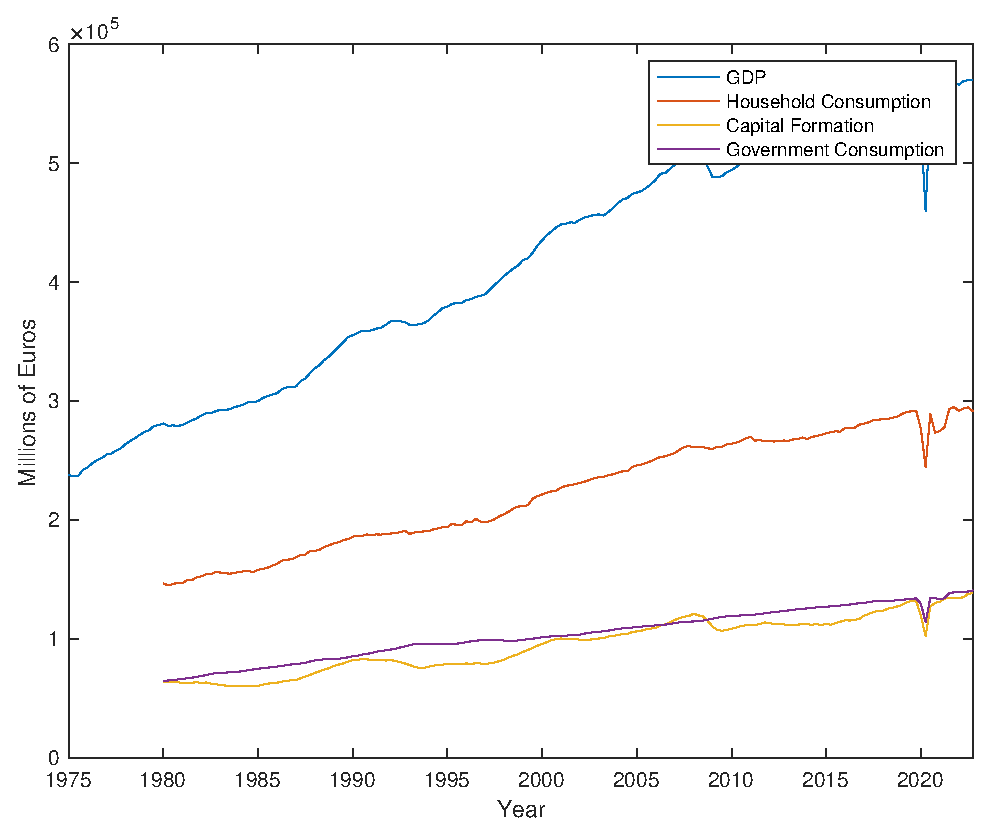
\includegraphics [width=4in]{Assignment_1_code_01.eps}


\subsection*{Comment: The time series plot for GDP, household consumption, government expenditure and investment shows the strong correlation between those time series. Consumption, investment, and government expenditure make up for about 52, 22 and 24 percent of GDP, respectively.}

\begin{verbatim}
%obtaining the stationary (cyclical) component using the HP filter and plot the cyclical components
lambda = 1600; % set the smoothing parameter
Y_cycle = hpfilter(log(Y), lambda);
C_cycle = hpfilter(log(C), lambda);
I_cycle = hpfilter(log(I), lambda);
G_cycle = hpfilter(log(G), lambda);
plot(Year, Y_cycle, Year, C_cycle, Year, I_cycle, Year, G_cycle);
xlabel('Year');
ylabel('Cyclical Component');
legend('GDP', 'Household Consumption', 'Capital Formation', 'Government Consumption');
\end{verbatim}

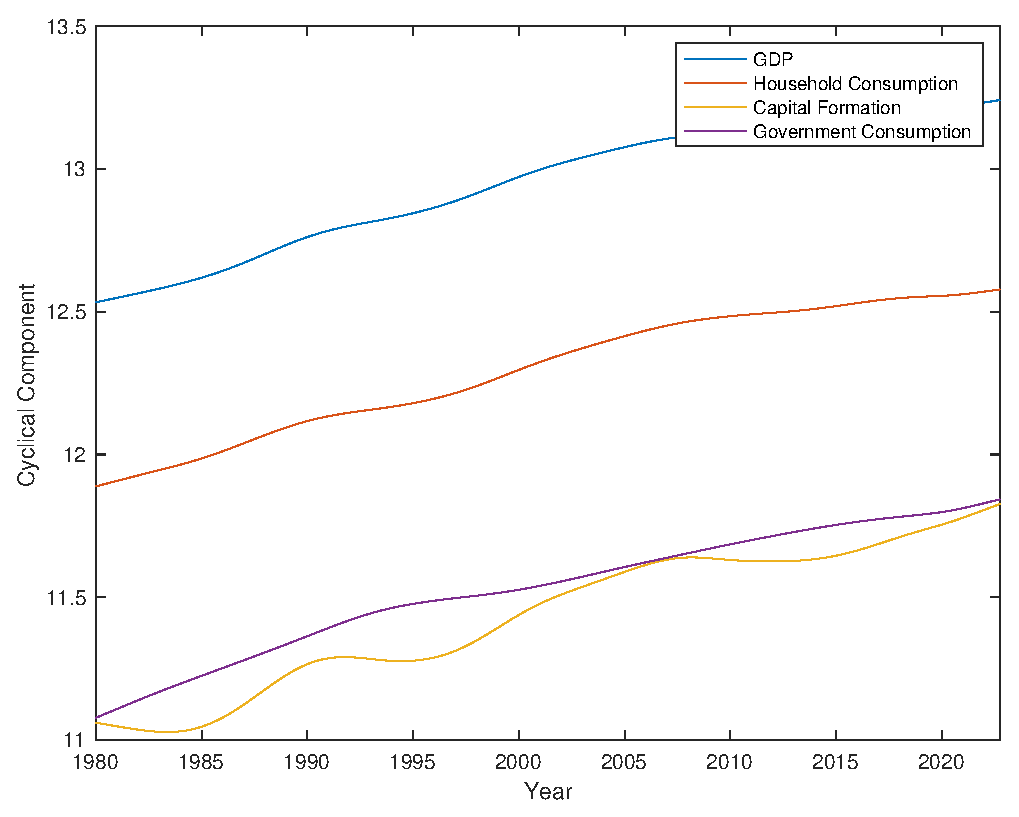
\includegraphics [width=4in]{Assignment_1_code_02.eps}


\subsection*{Comment: The stationary (cyclical) component of GDP, consumption, investment, and government expenditure is obtained using the HP filter with a smoothing parameter of 1600. The cyclical components for each variable are then plotted on the same graph. The plot shows how each variable deviates from its long-term trend over time. The cyclical component is much smoother than the original time series and captures the long-term trends in the data. From the curves, it appears that investments is the most volatile time series among the four.}

\begin{verbatim}
%creating summary table of business cycle stylized facts (full sample)
std_Y_cycle = std(Y_cycle);
std_C_cycle = std(C_cycle);
std_I_cycle = std(I_cycle);
std_G_cycle = std(G_cycle);
fprintf('Standard deviations of cyclical components:\n');
fprintf('Y_cycle: %.4f\n', std_Y_cycle);
fprintf('C_cycle: %.4f\n', std_C_cycle);
fprintf('I_cycle: %.4f\n', std_I_cycle);
fprintf('G_cycle: %.4f\n', std_G_cycle);
Y_rsd = std(Y_cycle) / mean(Y_cycle) * 100;
C_rsd = std(C_cycle) / mean(C_cycle) * 100;
I_rsd = std(I_cycle) / mean(I_cycle) * 100;
G_rsd = std(G_cycle) / mean(G_cycle) * 100;
fprintf('Relative Standard Deviations:\n');
fprintf('Y_cycle: %.4f%%\n', Y_rsd);
fprintf('C_cycle: %.4f%%\n', C_rsd);
fprintf('I_cycle: %.4f%%\n', I_rsd);
fprintf('G_cycle: %.4f%%\n', G_rsd);
corr_cyclical = corrcoef([Y_cycle, C_cycle, I_cycle, G_cycle]);
corr_matrix = corrcoef([Y_cycle, C_cycle, I_cycle, G_cycle]);
disp('Contemporaneous Output Correlations of Cyclical Components')
disp('---------------------------------------------------------')
disp('          Y         C         I         G')
disp(corr_matrix)
T = table(std_Y_cycle, std_C_cycle, std_I_cycle, std_G_cycle, Y_rsd, C_rsd, I_rsd, G_rsd, ...
          corr_matrix(1,1), corr_matrix(1,2), corr_matrix(1,3), corr_matrix(1,4), ...
          corr_matrix(2,1), corr_matrix(2,2), corr_matrix(2,3), corr_matrix(2,4), ...
          corr_matrix(3,1), corr_matrix(3,2), corr_matrix(3,3), corr_matrix(3,4), ...
          corr_matrix(4,1), corr_matrix(4,2), corr_matrix(4,3), corr_matrix(4,4), ...
          'VariableNames', {'Std_Y', 'Std_C', 'Std_I', 'Std_G', 'RSD_Y', 'RSD_C', 'RSD_I', 'RSD_G', ...
                            'Corr_Y_Y', 'Corr_Y_C', 'Corr_Y_I', 'Corr_Y_G', ...
                            'Corr_C_Y', 'Corr_C_C', 'Corr_C_I', 'Corr_C_G', ...
                            'Corr_I_Y', 'Corr_I_C', 'Corr_I_I', 'Corr_I_G', ...
                            'Corr_G_Y', 'Corr_G_C', 'Corr_G_I', 'Corr_G_G'});

disp(T)
\end{verbatim}

        \color{lightgray} \begin{verbatim}Standard deviations of cyclical components:
Y_cycle: 0.2208
C_cycle: 0.2156
I_cycle: 0.2438
G_cycle: 0.2112
Relative Standard Deviations:
Y_cycle: 1.7054%
C_cycle: 1.7531%
I_cycle: 2.1316%
G_cycle: 1.8319%
Contemporaneous Output Correlations of Cyclical Components
---------------------------------------------------------
          Y         C         I         G
    1.0000    0.9985    0.9921    0.9913
    0.9985    1.0000    0.9924    0.9900
    0.9921    0.9924    1.0000    0.9786
    0.9913    0.9900    0.9786    1.0000

     Std_Y      Std_C      Std_I      Std_G     RSD_Y     RSD_C     RSD_I     RSD_G     Corr_Y_Y    Corr_Y_C    Corr_Y_I    Corr_Y_G    Corr_C_Y    Corr_C_C    Corr_C_I    Corr_C_G    Corr_I_Y    Corr_I_C    Corr_I_I    Corr_I_G    Corr_G_Y    Corr_G_C    Corr_G_I    Corr_G_G
    _______    _______    _______    _______    ______    ______    ______    ______    ________    ________    ________    ________    ________    ________    ________    ________    ________    ________    ________    ________    ________    ________    ________    ________

    0.22085    0.21558    0.24376    0.21121    1.7054    1.7531    2.1316    1.8319       1        0.99847     0.99211     0.99132     0.99847        1        0.99241     0.99003     0.99211     0.99241        1        0.97858     0.99132     0.99003     0.97858        1    

\end{verbatim} \color{black}
    

\subsection*{Comment: The results indicate that the cyclical components of output (Y), consumption (C), investment (I), and government spending (G) have standard deviations ranging from 0.2112 to 0.2438, and relative standard deviations ranging from 1.7054\% to 2.1316\%. The contemporaneous output correlations of cyclical components suggest that there are high positive correlations among Y, C, I, and G, with correlation coefficients ranging from 0.9786 to 1.0000. This indicates that the cyclical fluctuations in these variables tend to move together. The relative standard deviation of investment is the highest among the four variables, at 2.1316\%. This suggests that investment is the most volatile of the four components. The relative standard deviation of consumption is slightly higher than that of output, at 1.7531\% and 1.7054\%, respectively. This suggests that consumption is also subject to some volatility, although less so than investment.}

\begin{verbatim}
% Splitting the data into two parts based on the date range
Y_cycle1 = Y_cycle(1:112,:);
C_cycle1 = C_cycle(1:112,:);
I_cycle1 = I_cycle(1:112,:);
G_cycle1 = G_cycle(1:112,:);
Y_cycle2 = Y_cycle(113:end,:);
C_cycle2 = C_cycle(113:end,:);
I_cycle2 = I_cycle(113:end,:);
G_cycle2 = G_cycle(113:end,:);

% Summary table for the "until 2007Q4" sample (hereafter called "subsample 1"
std_Y_cycle1 = std(Y_cycle1);
std_C_cycle1 = std(C_cycle1);
std_I_cycle1 = std(I_cycle1);
std_G_cycle1 = std(G_cycle1);
fprintf('Standard deviations of cyclical components for subsample 1:\n');
fprintf('Y_cycle: %.4f\n', std_Y_cycle1);
fprintf('C_cycle: %.4f\n', std_C_cycle1);
fprintf('I_cycle: %.4f\n', std_I_cycle1);
fprintf('G_cycle: %.4f\n', std_G_cycle1);
Y_rsd1 = std(Y_cycle1) / mean(Y_cycle1) * 100;
C_rsd1 = std(C_cycle1) / mean(C_cycle1) * 100;
I_rsd1 = std(I_cycle1) / mean(I_cycle1) * 100;
G_rsd1 = std(G_cycle1) / mean(G_cycle1) * 100;
fprintf('Relative Standard Deviations for subsample 1:\n');
fprintf('Y_cycle: %.4f%%\n', Y_rsd1);
fprintf('C_cycle: %.4f%%\n', C_rsd1);
fprintf('I_cycle: %.4f%%\n', I_rsd1);
fprintf('G_cycle: %.4f%%\n', G_rsd1);
corr_matrix1 = corrcoef([Y_cycle1, C_cycle1, I_cycle1, G_cycle1]);
disp('Contemporaneous Output Correlations of Cyclical Components for subsample 1')
disp('-----------------------------------------------------------------------')
disp('          Y         C         I         G')
disp(corr_matrix1)
T1 = table(std_Y_cycle1, std_C_cycle1, std_I_cycle1, std_G_cycle1, Y_rsd1, C_rsd1, I_rsd1, G_rsd1, ...
          corr_matrix1(1,1), corr_matrix1(1,2), corr_matrix1(1,3), corr_matrix1(1,4), ...
          corr_matrix1(2,1), corr_matrix1(2,2), corr_matrix1(2,3), corr_matrix1(2,4), ...
          corr_matrix1(3,1), corr_matrix1(3,2), corr_matrix1(3,3), corr_matrix1(3,4), ...
          corr_matrix1(4,1), corr_matrix1(4,2), corr_matrix1(4,3), corr_matrix1(4,4), ...
          'VariableNames', {'Std_Y', 'Std_C', 'Std_I', 'Std_G', 'RSD_Y', 'RSD_C', 'RSD_I', 'RSD_G', ...
                            'Corr_Y_Y', 'Corr_Y_C', 'Corr_Y_I', 'Corr_Y_G', ...
                            'Corr_C_Y', 'Corr_C_C', 'Corr_C_I', 'Corr_C_G', ...
                            'Corr_I_Y', 'Corr_I_C', 'Corr_I_I', 'Corr_I_G', ...
                            'Corr_G_Y', 'Corr_G_C', 'Corr_G_I', 'Corr_G_G'});
disp(T1)
\end{verbatim}

        \color{lightgray} \begin{verbatim}Standard deviations of cyclical components for subsample 1:
Y_cycle: 0.1801
C_cycle: 0.1684
I_cycle: 0.1944
G_cycle: 0.1632
Relative Standard Deviations for subsample 1:
Y_cycle: 1.4035%
C_cycle: 1.3830%
I_cycle: 1.7198%
G_cycle: 1.4305%
Contemporaneous Output Correlations of Cyclical Components for subsample 1
-----------------------------------------------------------------------
          Y         C         I         G
    1.0000    0.9983    0.9877    0.9831
    0.9983    1.0000    0.9905    0.9787
    0.9877    0.9905    1.0000    0.9542
    0.9831    0.9787    0.9542    1.0000

     Std_Y      Std_C      Std_I      Std_G     RSD_Y     RSD_C    RSD_I     RSD_G     Corr_Y_Y    Corr_Y_C    Corr_Y_I    Corr_Y_G    Corr_C_Y    Corr_C_C    Corr_C_I    Corr_C_G    Corr_I_Y    Corr_I_C    Corr_I_I    Corr_I_G    Corr_G_Y    Corr_G_C    Corr_G_I    Corr_G_G
    _______    _______    _______    _______    ______    _____    ______    ______    ________    ________    ________    ________    ________    ________    ________    ________    ________    ________    ________    ________    ________    ________    ________    ________

    0.18006    0.16839    0.19437    0.16324    1.4035    1.383    1.7198    1.4305       1        0.99831     0.98766     0.98313     0.99831        1        0.99048     0.97869     0.98766     0.99048        1        0.95424     0.98313     0.97869     0.95424        1    

\end{verbatim} \color{black}
    

\subsection*{Comment: The subsample analysis shows that cyclical components of output, consumption, investment, and government spending are highly correlated, with output and consumption being almost perfectly correlated. The relative standard deviation of the cyclical components for each variable is around 1.4\%. Compared to the results of the full sample, the subsample analysis shows a slightly lower degree of cyclical volatility.}

\begin{verbatim}
% Summary table for the "from 2008Q1" sample (hereafter called "subsample 2"
std_Y_cycle2 = std(Y_cycle2);
std_C_cycle2 = std(C_cycle2);
std_I_cycle2 = std(I_cycle2);
std_G_cycle2 = std(G_cycle2);
fprintf('Standard deviations of cyclical components for subsample 2:\n');
fprintf('Y_cycle: %.4f\n', std_Y_cycle2);
fprintf('C_cycle: %.4f\n', std_C_cycle2);
fprintf('I_cycle: %.4f\n', std_I_cycle2);
fprintf('G_cycle: %.4f\n', std_G_cycle2);
Y_rsd1 = std(Y_cycle2) / mean(Y_cycle2) * 100;
C_rsd1 = std(C_cycle2) / mean(C_cycle2) * 100;
I_rsd1 = std(I_cycle2) / mean(I_cycle2) * 100;
G_rsd1 = std(G_cycle2) / mean(G_cycle2) * 100;
fprintf('Relative Standard Deviations for subsample 2:\n');
fprintf('Y_cycle: %.4f%%\n', Y_rsd1);
fprintf('C_cycle: %.4f%%\n', C_rsd1);
fprintf('I_cycle: %.4f%%\n', I_rsd1);
fprintf('G_cycle: %.4f%%\n', G_rsd1);
corr_matrix1 = corrcoef([Y_cycle2, C_cycle2, I_cycle2, G_cycle2]);
disp('Contemporaneous Output Correlations of Cyclical Components for subsample 2')
disp('-----------------------------------------------------------------------')
disp('          Y         C         I         G')
disp(corr_matrix1)
T2 = table(std_Y_cycle2, std_C_cycle2, std_I_cycle2, std_G_cycle2, Y_rsd1, C_rsd1, I_rsd1, G_rsd1, ...
          corr_matrix1(1,1), corr_matrix1(1,2), corr_matrix1(1,3), corr_matrix1(1,4), ...
          corr_matrix1(2,1), corr_matrix1(2,2), corr_matrix1(2,3), corr_matrix1(2,4), ...
          corr_matrix1(3,1), corr_matrix1(3,2), corr_matrix1(3,3), corr_matrix1(3,4), ...
          corr_matrix1(4,1), corr_matrix1(4,2), corr_matrix1(4,3), corr_matrix1(4,4), ...
          'VariableNames', {'Std_Y', 'Std_C', 'Std_I', 'Std_G', 'RSD_Y', 'RSD_C', 'RSD_I', 'RSD_G', ...
                            'Corr_Y_Y', 'Corr_Y_C', 'Corr_Y_I', 'Corr_Y_G', ...
                            'Corr_C_Y', 'Corr_C_C', 'Corr_C_I', 'Corr_C_G', ...
                            'Corr_I_Y', 'Corr_I_C', 'Corr_I_I', 'Corr_I_G', ...
                            'Corr_G_Y', 'Corr_G_C', 'Corr_G_I', 'Corr_G_G'});
disp(T2)
\end{verbatim}

        \color{lightgray} \begin{verbatim}Standard deviations of cyclical components for subsample 2:
Y_cycle: 0.0391
C_cycle: 0.0327
I_cycle: 0.0640
G_cycle: 0.0517
Relative Standard Deviations for subsample 2:
Y_cycle: 0.2969%
C_cycle: 0.2611%
I_cycle: 0.5475%
G_cycle: 0.4401%
Contemporaneous Output Correlations of Cyclical Components for subsample 2
-----------------------------------------------------------------------
          Y         C         I         G
    1.0000    0.9982    0.9178    0.9900
    0.9982    1.0000    0.9046    0.9924
    0.9178    0.9046    1.0000    0.8785
    0.9900    0.9924    0.8785    1.0000

     Std_Y       Std_C       Std_I       Std_G      RSD_Y      RSD_C      RSD_I      RSD_G     Corr_Y_Y    Corr_Y_C    Corr_Y_I    Corr_Y_G    Corr_C_Y    Corr_C_C    Corr_C_I    Corr_C_G    Corr_I_Y    Corr_I_C    Corr_I_I    Corr_I_G    Corr_G_Y    Corr_G_C    Corr_G_I    Corr_G_G
    ________    ________    ________    _______    _______    _______    _______    _______    ________    ________    ________    ________    ________    ________    ________    ________    ________    ________    ________    ________    ________    ________    ________    ________

    0.039122    0.032702    0.063977    0.05172    0.29695    0.26113    0.54754    0.44013       1        0.99821     0.91776     0.99002     0.99821        1        0.90462     0.99243     0.91776     0.90462        1        0.87846     0.99002     0.99243     0.87846        1    

\end{verbatim} \color{black}
    

\subsection*{Comment: For subsample 2, the standard deviations of cyclical components are much lower than both the full sample and subsample 1. The relative standard deviations are also much lower for subsample 2. The contemporaneous output correlations of cyclical components for subsample 2 show higher correlation between Y and G compared to subsample 1, but lower correlation between Y and I. Overall, subsample 2 shows much lower volatility and correlation compared to the full sample and subsample 1.}

\begin{verbatim}
save('my_workspace.mat')
\end{verbatim}



\end{document}

